\documentclass[english,serif,mathserif,xcolor=pdftex,dvipsnames,table]{beamer}

\usepackage[T1]{fontenc}
\usepackage[utf8]{inputenc}

\usetheme[informal]{s3it}
\usepackage{s3it}

\title[Introduction to Python]{%
  A Short and Incomplete Introduction to Python
}
\subtitle{\bfseries Part 11: Ending remarks}
\author[S.~Haug]{%
  \textbf{Sigve Haug} \texttt{<sigve.haug@math.unibe.ch>}, \\
  Alexander Kashev \texttt{<alexander.kashev@math.unibe.ch>} \\
  Science IT Support (ScITS), University of Bern \\
  \medskip
  Based on a course by Riccardo Murri / Sergio Maffioletti
  \\
  S3IT: Services and Support for Science IT, UZH
}
\date{August 20--21, 2018}


\begin{document}

% title frame
\maketitle



\begin{frame}
  \frametitle{There is more to Python than this\ldots}

  The time and scope of this course is quite limited.

  \+
  Here is an (incomplete) list of Python features that you might
  want to look up as you become more experienced in the language:
  % XXX: mettere un link per ciascuna di queste!
  \begin{itemize}
  \item \href{https://github.com/gc3-uzh-ch/python-course}{Object-oriented progreamming}
  \item
    \href{http://docs.python.org/2/tutorial/classes.html\#iterators}{Iterators}
  \item
    \href{http://www.artima.com/weblogs/viewpost.jsp?thread=240808}{Decorators}
  \item \href{http://docs.python.org/2/tutorial/classes.html\#generators}{Generators}
  \item Class-level attributes, \href{http://stackoverflow.com/a/12179752/1808780}{classmethods, staticmethods}
  \item Properties and accessors
  \item \href{http://stackoverflow.com/a/6581949/459543}{Metaclasses}
  \end{itemize}
\end{frame}


\begin{frame}
  \frametitle{Want even more? Look into PyPI}
  \small

  \href{http://pypi.python.org}{PyPI} is \emph{the} index of Python software packages.
  It currently indexes 141'120 packages, so the choice is really vast.

  \begin{center}
    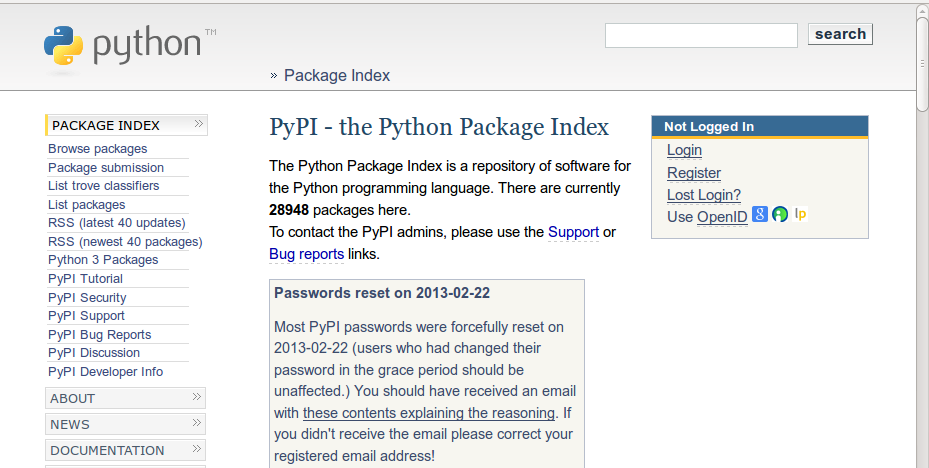
\includegraphics[width=0.60\textwidth]{fig/pypi_screenshot.png}
  \end{center}

  Almost all packages can be installed with a single command by
  running \href{https://pypi.python.org/pypi/pip}{\texttt{pip install
    \emph{packagename}}}.

\end{frame}


\begin{frame}
  \frametitle{Further reading}

  \begin{itemize}
    \item \textbf{The Python tutorial},
      {\small \url{http://docs.python.org/tutorial/}}
    \item {The Zen of Python in 3 days},
      {\small \url{http://pixelmonkey.org/pub/python-training/}}
  \end{itemize}

  \+   For an extensive and commented list, see:
  {\url{http://python-guide-pt-br.readthedocs.io/}}
\end{frame}

\begin{frame}
  \frametitle{Further reading}

  Nicolas Rougier has written excellent tutorials on the use of Matplotlib and NumPy:
  \begin{itemize}
  \item
    \url{https://www.labri.fr/perso/nrougier/teaching/matplotlib/} (Matplotlib tutorial)
  \item
    \url{http://www.labri.fr/perso/nrougier/teaching/numpy/numpy.html} (NumPy tutorial)
  \end{itemize}

  \+
  The Seaborn library comes with a good tutorial written by its author (note
  that -since Seaborn is an add-on to Matplotlib- some knowledge of Matplotlib
  is assumed): \url{http://seaborn.pydata.org/tutorial.html}
\end{frame}

% \begin{frame}
%   \begin{quote}
%     ``Reverend fathers, my letters were not wont either to be so prolix, or to
%     follow so closely on one another. Want of time must plead my excuse for both
%     of these faults. The present letter is a very long one, simply because I had
%     no leisure to make it shorter.''
%   \end{quote}

%   \+
%   {\small\em
%     Blaise Pascal, The Provincial Letters,
%     \href{https://ebooks.adelaide.edu.au/p/pascal/blaise/p27pr/part17.html}{Letter XVI}}
% \end{frame}


% \begin{frame}
%   \begin{quote}
%     ``Mes Révérends Pères, mes Lettres n'avaient pas accoutumé de se suivre de
%     si près, ni d'être si étendues. Le peu de temps que j'ai eu a été cause de
%     l'un et de l'autre. Je n'ai fait celle-ci plus longue que parce que je n'ai
%     pas eu le loisir de la faire plus courte.''
%   \end{quote}

%   \+
%   \begin{flushright}
%     \small\em
%     --- Blaise Pascal, \\
%     \href{https://www.ebooksgratuits.com/ebooksfrance/pascal_les_provinciales.pdf}{Seizième
%       lettre aux révérends pères jésuites}
%   \end{flushright}
% \end{frame}



\end{document}

%%% Local Variables:
%%% mode: latex
%%% TeX-master: t
%%% End:
